\section{Lineare Least-Squares Regression mit Regularisierung in Python}


\subsection{
    Betrachtung des Programmgerüst \textit{V2A1\textunderscore LinearRegression.py}
}

\subsubsection{Erklärung der Funktionen: \textit{fun\textunderscore true(), generateDataSet(), getDataError(), phi\textunderscore polynomial()}}

\textbf{fun\textunderscore true():} Berechnet die Funktionswerte der Parabel
$y(x) = w0 + w1*x + w2*x$. Die X-Werte werden als Nx1-dimensionales np.array übergeben.

\vspace{5px}
\noindent
\textbf{generateDataset():} Fügt den von \textit{fun\textunderscore true()} berechneten Funktionswerten ein Rauschen hinzu. Rückgabewerte sind die X-Werte sowie die Funktionswerte T mit Rauschen.

\vspace{5px}
\noindent
\textbf{getDataError():} Berechnet die Datenfehler (Least Squares) zwischen Vorhersagedaten und den aus \textit{generateDataSet()} erzeugten \textit{True Target-Werten}.

\vspace{5px}
\noindent
\textbf{phi\textunderscore polinomial():} Generiert jeweils einen Merkmalsvektor phi\textunderscore x. In anderen Worten eine Zeile der Designmatrix PHI.

\subsubsection{Von welcher Funktion sind die Original-Daten (xn, tn) gesampelt?}

Die Python-Funktion \textit{fun\textunderscore true()} sampelt die Daten anhand der mathematischen Funktion $y(x) = w0 + w1*x + w2*x$.

\subsubsection{Wie lauten die Basisfunktionen $phi\textunderscore j(x)$ für j = 1, ..., deg des linearen Modells?}

$phi\textunderscore j (x) = \begin{smallmatrix}(1&x&x^2&x^3&...&x^\mathrm{deg})\end{smallmatrix}$
Die Basisfunktion kann durch die Variable \textit{deg} angepasst werden.

\subsubsection{Welche Rolle hat die Variable lambda?}
Durch geeignete Wahl von lmbda kann man die Überanpassung vermeiden.
Dient demnach zur Regularisierung.

\subsubsection{Worin unterscheiden sich die Variablen X,T von X\textunderscore test,T\textunderscore test?}
Um die Qualität der ermittelten Regressions-Funktion zu prüfen, werden Trainingsdaten von Testdaten getrennt.

\subsubsection{Was stellen im Plot die grünen Kreuze/Punkte, grüne Kurve, rote Kurve dar?}
\textbf{Grüne Punkte:} stellen die generierten Testdatenpunkte dar.\\
\textbf{Grüne Kreuze:} stellen die generierten Datenpunkte dar.\\
\textbf{Grüne Kurve:} stellt die ursprüngliche Parabel-Funktion dar.\\
\textbf{Rote Kurve:} stellt die ermittelte Trennkurve dar.

\subsection{Vervollständigung des Programm}

\subsubsection{Implementierung der Berechnung der regularisierten Least-Squares-Gewichte W\textunderscore LSR als M x 1-Matrix}

\begin{figure}[H]
    \centering
    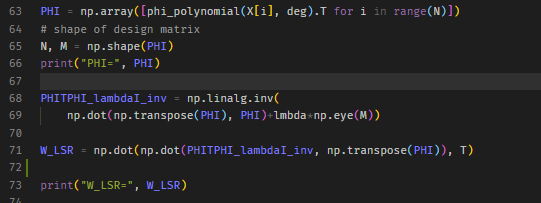
\includegraphics[width=1\linewidth]{sections/v2a1_wlsr_impl.png}
    \caption{Least-Squares-Gewichte}
\end{figure}

\subsubsection{Implementierung der Berechnung der Prognosewerte Y als N x 1-Matrix}

\begin{figure}[H]
    \centering
    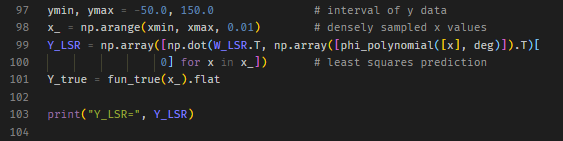
\includegraphics[width=1\linewidth]{sections/v2a1_y_impl.png}
    \caption{Berechnung der Prognosefunktion}
\end{figure}

\subsection{Programmtest ohne Regularisierung}

\begin{figure}[H]
    \centering
    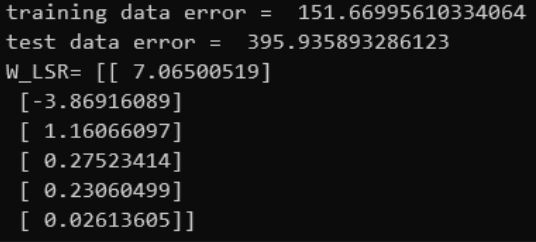
\includegraphics[width=1\linewidth]{sections/v2a1c1.png}
    \caption{Test ohne Regularisierung}
\end{figure}

Aus der vorherigen Abbildung können die optimalen Gewichte $W_mathrm{LSR}$,
der Lerndaten- sowie der Testdaten-Fehler entnommen werden. Der Testdaten-Fehler ist deutlich höher, dies liegt vermutlich am Overfitting. Der Polynomgrad 5 bietet anscheinend zu viele Freiheitsgrade.

\subsubsection{Phänomene bei niedrigem bzw. hohem Polynomgrad}
Vergleicht man die Lern- und Test-Datenfehler für verschiedene Polynomgrade erkennt man, dass bei einem zu niedrigen Polynomgrad (1, 2) die Funktion zu unflexibel ist und beide Datenfehler groß sind. Bei einem zu hohen Polynomgrad ist zwar der Lern-Datenfehler geringer, jedoch der Test-Datenfehler groß auf Grund von Overfitting.

\subsubsection{Bestimmung des mittleren Gewichts für versch. Polynomgrade}

\begin{figure}[H]
    \centering
    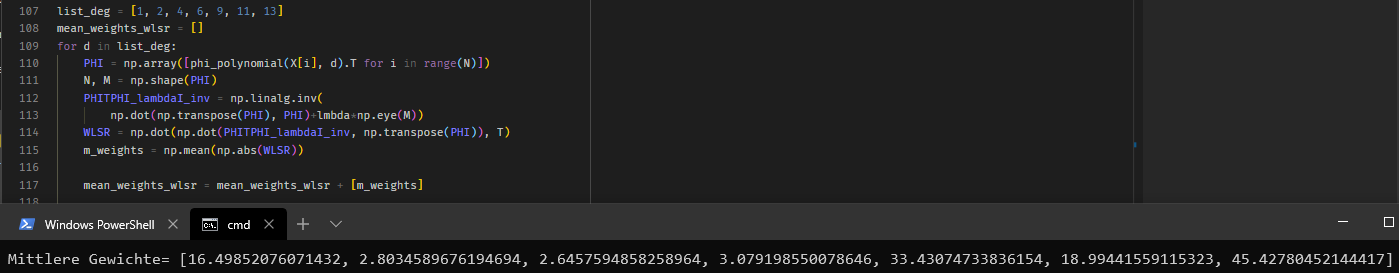
\includegraphics[width=1\linewidth]{sections/v2a1c3.png}
    \caption{Mittlere Gewichte zu versch. Polynomgraden}
\end{figure}

\subsubsection{Lern- bzw. Test-Datenfehler pro Datenpunkt für versch. große Datensets}

\begin{figure}[H]
    \centering
    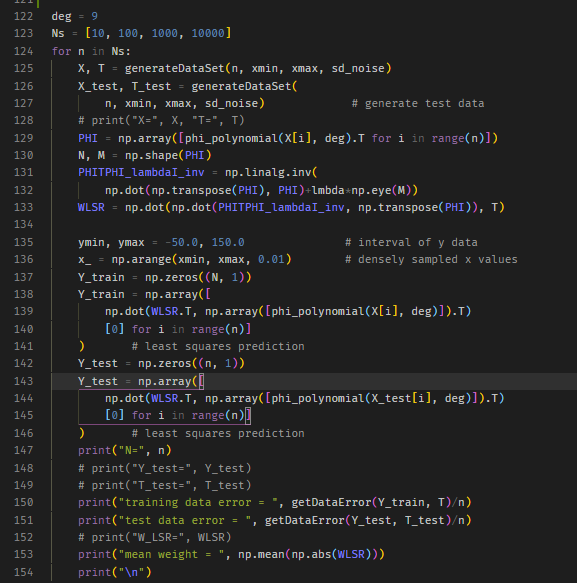
\includegraphics[width=1\linewidth]{sections/v2a1c4.png}
    \caption{Implementierung}
\end{figure}

\begin{figure}[H]
    \centering
    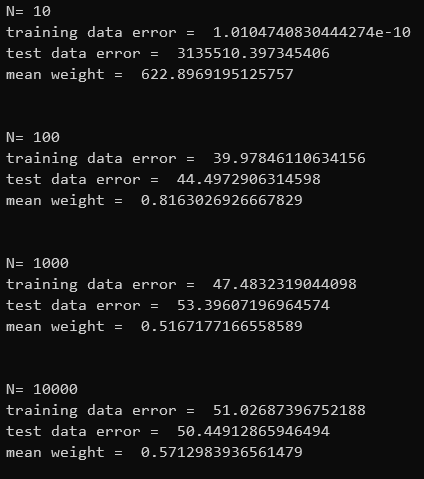
\includegraphics[width=1\linewidth]{sections/v2a1c4_result.png}
    \caption{Lern- und Test-Datenfehler versch. großer Datensets}
\end{figure}

Bei gleichbleibendem Polynomgrad und größeren Datensets nimmt der Lern-Datenfehler zu. Der Test-Datenfehler nimmt deutlich ab, jedoch nur bis zu einem bestimmten Punkt.
